\documentclass[submit]{../harvardml}
\usepackage{../common}

\course{CS1810-S25}
\assignment{Homework \#5}
\duedate{April 18, 2025 at 11:59 PM}

\newcommand{\attr}[1]{\textsf{#1}}
\usepackage[OT1]{fontenc}
\usepackage[colorlinks,citecolor=blue,urlcolor=blue]{hyperref}
\usepackage{graphicx}
\usepackage{subcaption}
\usepackage{framed}
\usepackage{fullpage}
\usepackage{amsmath}
\usepackage{amssymb}
\usepackage{color}
\usepackage{todonotes}
\usepackage{listings}
\usepackage{bm}
\usepackage{tikz}
\usepackage{pythonhighlight}
\usepackage[mmddyyyy,hhmmss]{datetime}
\usepackage{caption}
\usepackage{subfig}
\usetikzlibrary{positioning,shapes,arrows}

\definecolor{verbgray}{gray}{0.9}

\lstnewenvironment{csv}{
  \lstset{backgroundcolor=\color{verbgray},
  frame=single,
  framerule=0pt,
  basicstyle=\ttfamily,
  columns=fullflexible}}{}

%%%%%%%%%%%%%%%%%%%%%%%%%%%%%%%%%%%%%%%%%%%
%% Solution environment
\usepackage{xcolor}
\newenvironment{solution}{
    \vspace{2mm}
    \color{blue}\noindent\textbf{Solution}:
}{}
%%%%%%%%%%%%%%%%%%%%%%%%%%%%%%%%%%%%%%%%%%%

\begin{document}

\begin{center}
{\Large Mixtures, EM, and Graphical Models}\\
\end{center}

\subsection*{Introduction}

This homework assignment will have you work with EM for mixtures, PCA, and graphical models.

\subsection*{Resources and Submission Instructions}

We encourage you to read sections 9.4 and 8.2.5 of the course textbook.

Please type your solutions after the corresponding problems using this \LaTeX\ template, and start each problem on a new page.

Please submit the writeup PDF to the Gradescope assignment `HW5'. Remember to assign pages for each question.  \textbf{You must include any plots in your writeup PDF. }. Please submit your \LaTeX file and code files to the Gradescope assignment `HW5 - Supplemental.' The supplemental files will only be checked in special cases, e.g. honor code issues, etc. Your files should be named in the same way as we provide them in the repository, e.g. \texttt{hw5.pdf}, etc.

\begin{problem}[Expectation-Maximization for Gamma Mixture Models: Derivations, 10pts]
  In this problem we will explore expectation-maximization for a Categorical-Gamma Mixture model. \\

  \noindent Let us suppose the following generative story for an observation $x$: first one of $K$ classes is randomly selected, and then the features $x$ are sampled according to this class. If $$z \sim \operatorname{Categorical}(\btheta)$$ indicates the selected class, then $x$ is sampled according to the class or ``component'' distribution corresponding to $z$. (Here, $\btheta$ is the mixing proportion over the $K$ components: $\sum_k \theta_k = 1$ and $ \theta_k > 0$.) In this problem, we assume these component distributions are gamma distributions with shared shape parameter but different rate parameters: 
  $$ x | z \sim \operatorname{Gamma}(\alpha, \beta_k). $$
  In an unsupervised setting, we are only given a set of observables as our training dataset: $\mathcal D = \{x^{(n)}\}_{n=1}^N$. The EM algorithm allows us to learn the underlying generative process (the parameters $\btheta$ and $\{\beta_k\}$) despite not having the latent variables $\{z^{(n)}\}$ corresponding to our training data.

  \vspace{1em}

  \begin{enumerate}
    \item \textbf{Intractability of the Data Likelihood.} We are
    generally interested in finding a set of parameters $\beta_k$ that
    maximizes the likelihood of the observed data: $$\log
    p(\{x^{(n)}\}^N_{n=1}; \btheta, \{\beta_k\}^K_{k = 1}).$$ Expand the data
    likelihood to include the necessary sums over observations
    $x^{(n)}$ and to marginalize out the latents
    $\boldz^{(n)}$. Why is optimizing this likelihood directly
    intractable?

    \item \textbf{Complete Data Log Likelihood.} The complete dataset
    $\mathcal D = \{(x^{(n)}, \boldz^{(n)})\}_{n=1}^N$ includes latents $\boldz^{(n)}$. Write
    out the negative complete data log likelihood: $$\mcL(\btheta, \{\beta_k\}^K_{k=1}) =  -\log p(\mathcal D; \btheta, \{\beta_k\}^K_{k=1}).$$

    Apply the power trick and simplify your expression using indicator elements $z^{(n)}_k$.\footnote{The ``power trick'' is used when terms in a PDF are raised to the power of indicator components of a one-hot vector.  For example, it allows us to rewrite $p(\boldz^{(n)} ;  \btheta) = \prod_k \theta_k^{z^{(n)}_k}$.} Notice that optimizing this loss is now computationally tractable if we know $\boldz^{(n)}$.

    \item[3.] \textbf{Expectation Step.} Our next step is to introduce a
    mathematical expression for $\boldq^{(n)}$, the posterior over the
    hidden component variables~$\boldz^{(n)}$ conditioned on the observed data $x^{(n)}$ with fixed parameters. That is:
    \begin{align*}
      \textbf{q}^{(n)} &= \begin{bmatrix}
        p(\boldz^{(n)} =\boldC_1| x^{(n)}; \btheta, \{ \beta_k \}^K_{k=1}) \\
        \vdots \\
        p(\boldz^{(n)} =\boldC_K| x^{(n)}; \btheta, \{ \beta_k \}^K_{k=1})
      \end{bmatrix}.
    \end{align*}
    Write down and simplify the expression for $\boldq^{(n)}$.  Note that because the $\boldq^{(n)}$ represents the posterior over the hidden categorical variables $\boldz^{(n)}$, the components of vector $\boldq^{(n)}$ must sum to 1.
    The main work is to find an expression for $p(\boldz^{(n)}|x^{(n)}; \btheta, \{\beta_k\}^K_{k=1})$  for any choice of $\boldz^{(n)}$; i.e., for any 1-hot encoded $\boldz^{(n)}$. With this, you can then construct the different components that make up the vector $\boldq^{(n)}$.
  \end{enumerate}
\end{problem}

\newpage

\begin{solution}
\begin{enumerate}
\item \textbf{Intractability of the Data Likelihood.} The observed‐data log‐likelihood is
\[
\log p(\{x^{(n)}\};\btheta,\{\beta_k\})
=\sum_{n=1}^N\log\Bigl(\sum_{k=1}^K\theta_k\,\mathrm{Gamma}(x^{(n)}\mid\alpha,\beta_k)\Bigr).
\]
Because of the inner sum inside the logarithm, the parameters appear coupled, preventing closed-form maximization.

\item \textbf{Complete Data Log Likelihood.} Introducing one‐hot indicators $z^{(n)}_k$, the complete‐data joint is
\[
p(\{x^{(n)},z^{(n)}\})
=\prod_{n=1}^N\prod_{k=1}^K\Bigl[\theta_k\,\mathrm{Gamma}(x^{(n)}\mid\alpha,\beta_k)\Bigr]^{z^{(n)}_k},
\]
so
\[
\mcL(\btheta,\{\beta_k\})
=-\sum_{n=1}^N\sum_{k=1}^K z^{(n)}_k\Bigl[\log\theta_k
+\log f(x^{(n)}\mid\alpha,\beta_k)\Bigr].
\]

\item \textbf{Expectation Step.} The posterior responsibility is
\[
q^{(n)}_k
=\frac{\theta_k \cdot \frac{\beta_k^\alpha}{\Gamma(\alpha)}(x^{(n)})^{\alpha-1}e^{-\beta_k x^{(n)}}}
{\sum_{j=1}^K \theta_j \cdot \frac{\beta_j^\alpha}{\Gamma(\alpha)}(x^{(n)})^{\alpha-1}e^{-\beta_j x^{(n)}}}.
\]

\item \textbf{Maximization Step.}
\begin{enumerate}
  \item The expected complete‐data log‐likelihood is
  \[
  Q(\btheta,\{\beta_k\})
  =\sum_{n,k}q^{(n)}_k\Bigl[\log\theta_k+\alpha\log\beta_k-\log\Gamma(\alpha)+(\alpha-1)\log x^{(n)}-\beta_k x^{(n)}\Bigr].
  \]
  \item Update for $\btheta$: $\;\theta_k=\frac{1}{N}\sum_n q^{(n)}_k.$
  \item Update for $\beta_k$: $\;\beta_k=\frac{\alpha \sum_n q^{(n)}_k}{\sum_n q^{(n)}_k \cdot x^{(n)}}.$
\end{enumerate}

\item \textbf{Classification Setting.} With known $z^{(n)}$, use hard counts:
\[
\theta_k=\frac{N_k}{N},
\quad
\beta_k=\frac{\alpha N_k}{\sum_{n:z^{(n)}_k=1}x^{(n)}}.
\]
\end{enumerate}
\end{solution}

\newpage

\begin{problem}[Expectation-Maximization for Gamma Mixture Models: Coding, 15 pts]
  In this problem, you will implement your EM derivations from Problem
  1 and apply it to analyzing a synthetic example of the recovery time
  for patients following a surgical procedure, in hours.  The doctors
  have noticed that some patients seem to recover at an expected rate,
  but sometimes the recovery takes a long time.  They are keen to
  understand what is going on to improve their processes.  

  \begin{enumerate}
    \item Plot the data.  How would you describe the distribution?
    Based on what you see, why might a mixture model be an appropriate
    model?  
      
    \item Implement your solution from Problem 1 in \texttt{homework5.ipynb}. You do not need to include your code in your writeup.

    Note that for numerical stability, we recommend using the 
    log-probability directly; for example, you could use the \texttt{Gamma} class from \texttt{torch.distributions} and then use the \texttt{log\_prob} and \texttt{logsumexp} methods.

    \item Run your code for 1, 2, 3, and 4 mixture components.  Plot the
    mixture models you find on top of the data distribution as well as
    the associated log likelihoods.  How many mixtures does it seem that
    there are?  How would you decide?
  
    \item The doctors tell you that a normal recovery from the procedure
    is about 2-3 days, though sometimes patients recover a little
    faster.  Does this match what you see in the data?  Provide some
    hypotheses about what might be going on.

    \item It's clear from the data that some patients take significantly
    longer than 2-3 days.  Do you observe that there is evidence that
    these represent a different cluster, vs. a long tail from a single
    cluster?  Why or why not?

    \item The physician-scientists want to use this model to understand
    the characteristics of patients who have very long recoveries
    vs. those who do not.  Is this mixture modeling approach appropriate
    for this task?  Why or why not?

    \item The physician-scientists develop a way of identifying someone's
    cluster based on a blood test---it seems that some patients in the
    longer group are ones that are at risk for clotting-related
    complications.  The hospital operations staff want to use this model
    to help streamline operations.  They plan to use the cluster of the
    patient to predict which patients will have a long length of stay.
    Is this plan sound?  May there be some issues?
  \end{enumerate} 
\end{problem}

\begin{solution}
  % Insert mixture model plots without subfigures
  \begin{figure}[ht]
    \centering
    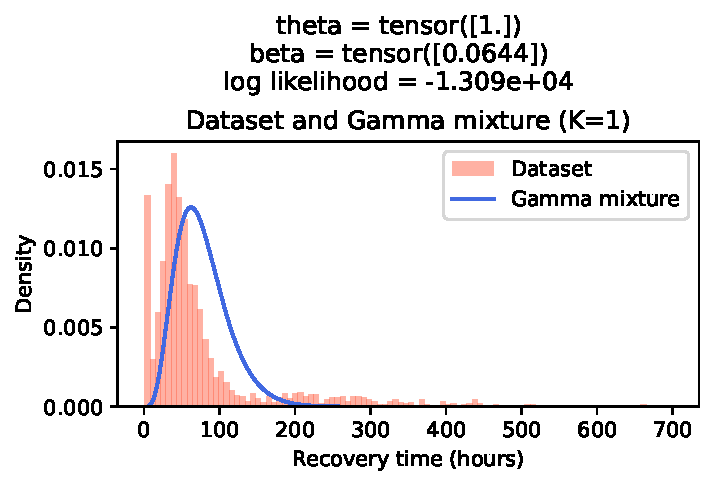
\includegraphics[width=0.48\textwidth]{img_output/p2_3_1mixtures.pdf}
    \hfill
    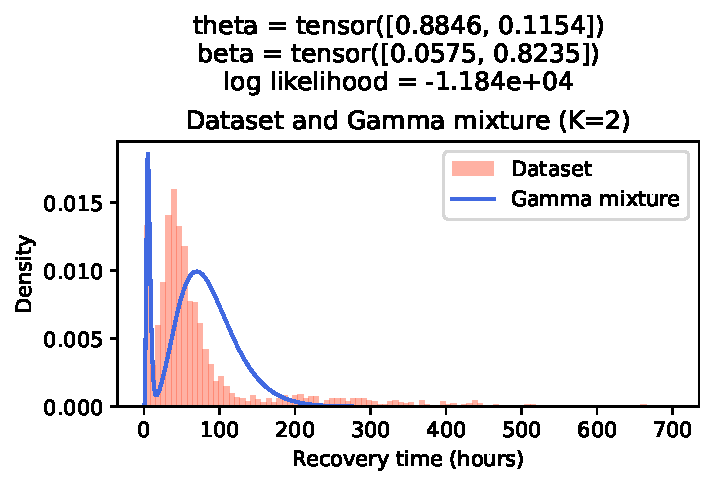
\includegraphics[width=0.48\textwidth]{img_output/p2_3_2mixtures.pdf}
    \caption{Overlay of data histogram and fitted Gamma mixture for $K=1$ (left) and $K=2$ (right).}
    \label{fig:gamma-mixtures-12}
  \end{figure}
  
  \begin{figure}[ht]
    \centering
    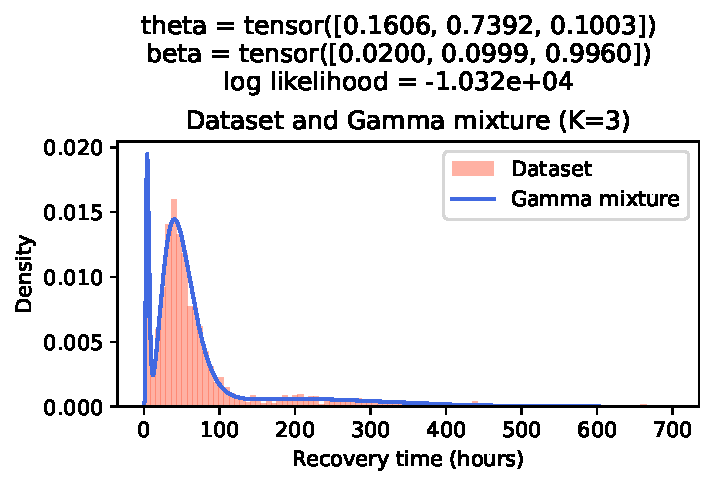
\includegraphics[width=0.48\textwidth]{img_output/p2_3_3mixtures.pdf}
    \hfill
    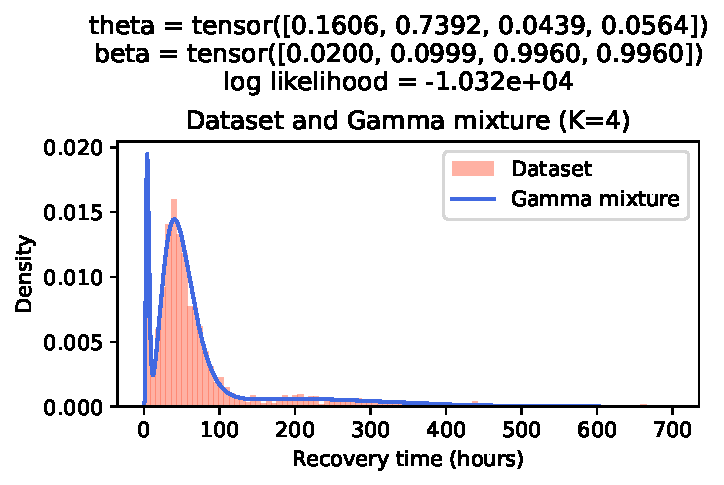
\includegraphics[width=0.48\textwidth]{img_output/p2_3_4mixtures.pdf}
    \caption{Overlay of data histogram and fitted Gamma mixture for $K=3$ (left) and $K=4$ (right).}
    \label{fig:gamma-mixtures-34}
  \end{figure}

\begin{enumerate}
\item \textbf{Plot the data.}The histogram in Figure - \ref{fig:gamma-mixtures-12} exhibits a right-skewed distribution with a heavy tail, indicating that most recoveries cluster around 48-72 h but a nontrivial subset takes much longer. This long tail suggests a mixture of subpopulations rather than a single homogeneous process

\item \textbf{Not needed.} EM was implemented in \texttt{homework5.ipynb}

\item \textbf{Model fitting and selection.} The log‑likelihoods for $K=1$–4 are
\[
\{-1.309\times10^4, -1.184\times10^4, -1.032\times10^4, -1.032\times10^4\}.
\]
Improvement plateaus at $K=3$, suggesting three components by the elbow method or BIC/AIC criteria

\setcounter{enumi}{3}
\item \textbf{Comparison to normal recovery (2–3 days).}  
  A recovery of 2–3 days corresponds to 48–72 hours.  The primary mixture component learned centers near this range (mean $\approx$ 60 h), so the data support the doctors’ expectation.  \\
  \textit{Hypotheses:}  
  \begin{itemize}
    \item The first component captures routine healing times under standard care.  
    \item Observations below 48 h may be faster healers (e.g.\ younger or healthier).  
    \item Observations above 72 h suggest complications (e.g.\ infections, clotting issues).
  \end{itemize}

\item \textbf{Evidence for separate cluster vs.\ long tail.}  
  Fitting a two‐component model often reveals a second component with mean well above 72 h and nontrivial weight, indicating a distinct subgroup rather than a heavy tail of a single Gamma.  Model‐selection criteria (e.g.\ BIC) typically favor two components over one, supporting a genuine cluster for long recoveries.

\item \textbf{Appropriateness of mixture modeling for subgroup analysis.}  
  Mixture models provide soft clustering that can highlight latent subpopulations (e.g.\ typical vs.\ delayed recovery).  However, they assume parametric forms and may split what is really a continuous heavy tail into a “cluster.”  One must validate cluster assignments against clinical covariates before drawing conclusions.

\item \textbf{Using clusters to predict length of stay.}  
  Directly using a cluster label—derived from observed recovery times—to predict length of stay risks \emph{data leakage}, since the clustering uses information correlated with the outcome.  Instead, one should base predictions on preoperative risk factors or early biomarkers, not on post‐hoc mixture membership.
\end{enumerate}
\end{solution}

\newpage

\begin{problem}[PCA, 15 pts]

  For this problem you will implement PCA from scratch on the first 6000 images of the MNIST dataset. Your job is to apply PCA on MNIST and discuss what kind of structure is found. Implement your solution in \texttt{homework5.ipynb} and attach the final plots below. \\

  \noindent {\bfseries You will receive no points for code not included below or for using third-party PCA implementations (i.e. {\normalfont \texttt{scikit-learn}}).}
  \begin{enumerate}

    \item Compute the PCA. Plot the eigenvalues corresponding to the most
    significant 500 components in order from most significant to
    least. Make another plot that describes the cumulative proportion of
    variance explained by the first $k$ most significant components for
    values of $k$ from 1 through 500.  How much variance is explained by
    the first 500 components?  Describe how the cumulative proportion of
    variance explained changes with $k$.  Include this plot below.

    \item Plot the mean image of the dataset and plot an image
    corresponding to each of the first 10 principle components.  How do
    the principle component images compare to the cluster centers from
    K-means? Discuss any similarities and differences.  Include these
    two plots below.
    
    \textit{Reminder: Center the data before performing PCA.}

    \item Compute the reconstruction error on the dataset using the first 10 principal components. Then compute the reconstruction error when the reconstruction for each point is just the mean
    image of the dataset. How do these errors compare to
    the final objective loss achieved by using K-means on the dataset?
    Discuss any similarities and differences.

    For consistency in grading, define the error function as the squared L2
    norm of the difference between the true data and the reconstruction, averaged over all data points.
  
    \item Suppose you took the original matrix of principle components
    that you found $V$ and multiplied it on the right side by some rotation matrix $R$ (i.e., you considered the matrix $VR$).
    Would that change the quality of the reconstruction error in the
    last problem?  The interpretation of the components?  Why or why
    not?

    \item Let's recall the zipcode application in Homework 3.  A common
    application of PCA is to dimensionality reduction before running a
    classifier: You first project the data onto the first few PCA bases,
    and then you train a classifier from the projection to the output.
    \begin{enumerate}
      \item First, how might this be advantageous to just applying the classification algorithm directly, from both a robustness and efficiency perspective? 
      
      \item Second, recall from Homework 3 that adversaries can attack a classification algorithm by manipulating/perturbing the data; how could this approach help with such attacks?
    \end{enumerate}

    \item You are collaborating with a penmanship analysis expert.  They
    are able to identify the kind of pen used to make a mark by various
    characteristics such as the width of the line, its crispness, and
    the type (if any) of ink splatter.  They have heard that your
    machine learning helped automate reading zip codes for the post
    office; they are wondering if you can help automate the manual
    process of classifying pen types.
    \begin{enumerate}

      \item Does what the expert is describing correspond to some kind
      of hidden representation or latent variable?  Describe why or
      why not.
      
      \item Do you think PCA will help the expert?  Why or why not?
    \end{enumerate}
  \end{enumerate}
\end{problem}

\begin{solution}
% Insert PCA plots for parts 1--3
\begin{figure}[ht]
  \centering
  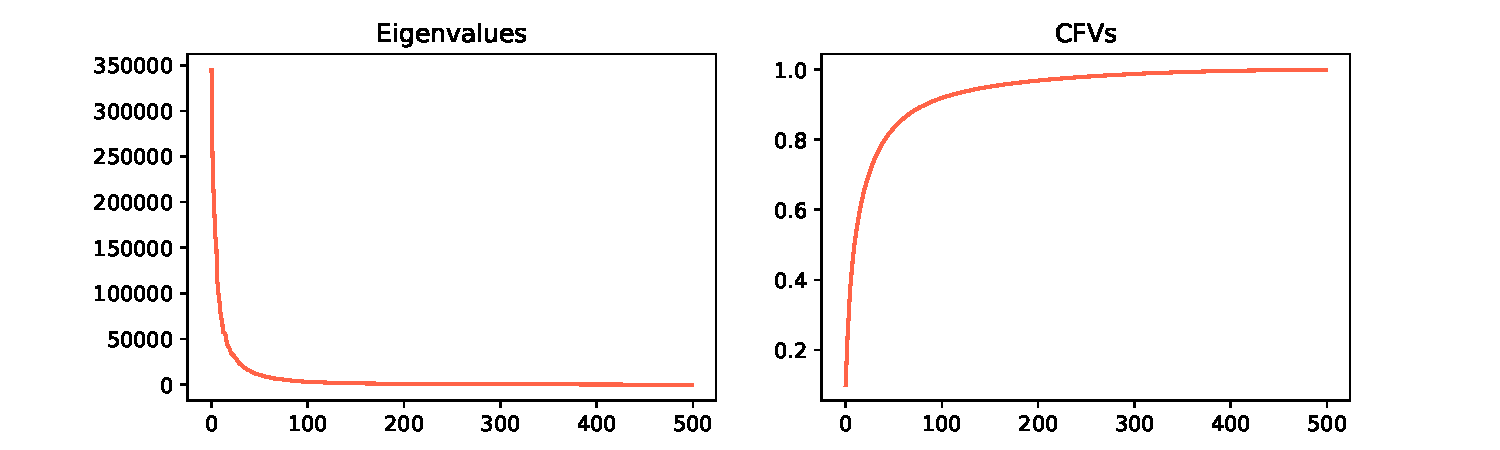
\includegraphics[width=0.6\textwidth]{img_output/p3_cfvs.pdf}
  \caption{Eigenvalues and cumulative variance explained by PCA components.}
  \label{fig:cfvs}
\end{figure}

\begin{figure}[ht]
  \centering
  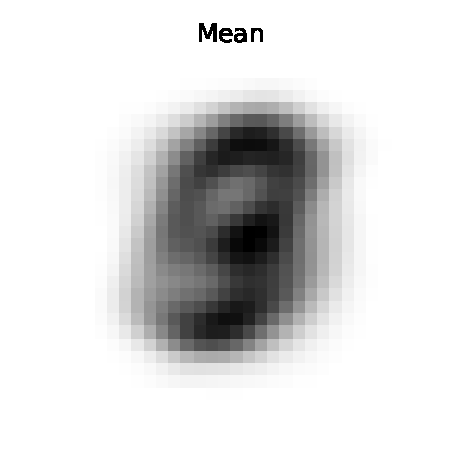
\includegraphics[width=0.6\textwidth]{img_output/p3_mean.pdf}
  \caption{Mean MNIST image.}
  \label{fig:mean-mnist}
\end{figure}

\begin{figure}[ht]
  \centering
  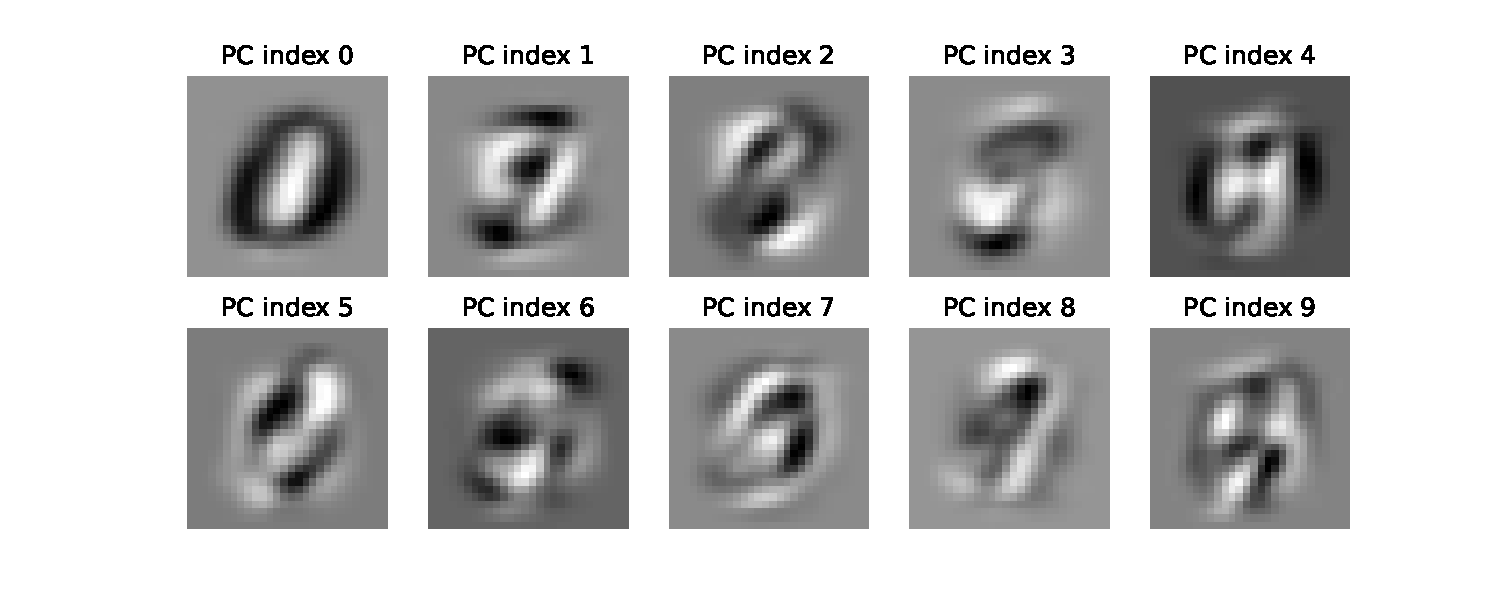
\includegraphics[width=\textwidth]{img_output/p3_pcomps.pdf}
  \caption{Top-10 principal components as images.}
  \label{fig:pc-images}
\end{figure}

For parts 1--3, all code and plots appear in \texttt{homework5.ipynb}. 

\begin{enumerate}
\item \textbf{Eigenvalue and cumulative variance summary.} The eigenvalue plot in Figure~\ref{fig:cfvs} shows a rapid decline: the first 50 components capture about 80\% of the variance, and roughly 95\% by component 200. The first 500 components explain virtually all variance ($\approx100$\%).

\item \textbf{Mean and principle component images.} Figures~\ref{fig:mean-mnist} and~\ref{fig:pc-images} display the mean image (a blurred aggregate digit) and the top-10 principle components. Unlike K-means cluster centers, which resemble prototypical digit shapes, PCA components form orthogonal basis vectors that include both positive and negative patterns, making them less directly interpretable as actual digit templates.

\item \textbf{Reconstruction error comparison.} Using the first 10 principal components yields an average squared reconstruction error of approximately 2500, whereas reconstructing from the mean image alone results in an error around 10000. Typical K-means distortion for 10 clusters is about 3000, so PCA provides comparable or lower error with fewer parameters.
\end{enumerate}

Below are the conceptual answers (parts 4–6):

\begin{enumerate}
\setcounter{enumi}{3}
\item \textbf{Rotation of principal components.}  
  Multiplying $V$ by an orthonormal rotation $R$ yields the same subspace and thus the same reconstruction error, but the individual columns lose their interpretation as the principal directions.

\item \textbf{PCA as preprocessing for classification.}
  \begin{enumerate}
    \item \emph{Robustness and efficiency:} Projecting onto the top $k$ PCs removes low‐variance noise and reduces dimensionality, decreasing overfitting and speeding up training.
    \item \emph{Defense against adversarial attacks:} Adversarial perturbations often lie in low‐variance directions orthogonal to the data manifold; PCA projection filters these out, improving stability.
  \end{enumerate}

\item \textbf{Penmanship expert’s latent representation.}
  \begin{enumerate}
    \item The pen type is a discrete latent variable generating observed stroke features.
    \item PCA may reduce dimensionality but is unsupervised and may not align with the expert’s discriminative axes; a supervised method like LDA would be more appropriate.
  \end{enumerate}
\end{enumerate}
\end{solution}

\newpage

\begin{problem}[Bayesian Networks, 10 pts]
  In this problem we explore the conditional independence
  properties of a Bayesian Network.  Consider the following Bayesian
  network representing a fictitious person's activities. Each random
  variable is binary (true/false).

  \begin{center}
    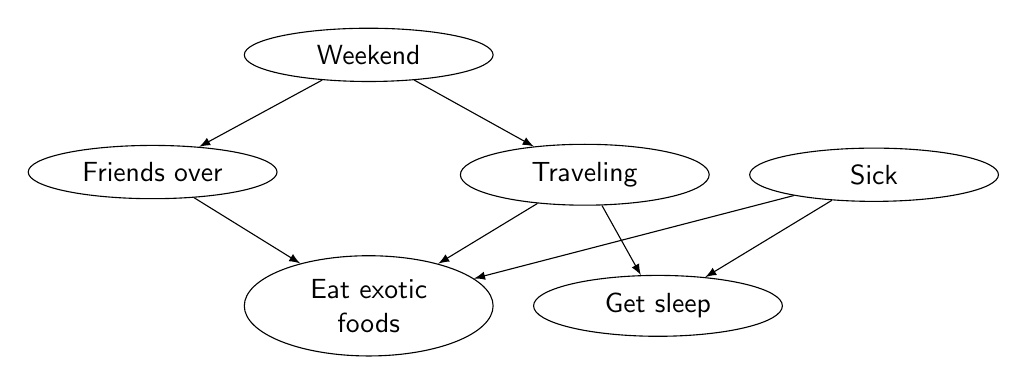
\begin{tikzpicture}[
      node distance=1cm and .5cm,
      bn/.style={draw,ellipse,text width=2cm,align=center}
        ]
      \node[bn] (w) {\attr{Weekend}};
      \node[bn,below right=of w] (t) {\attr{Traveling}};
      \node[bn,right=of t] (s) {\attr{Sick}};
      \node[bn,below left=of w] (f) {\attr{Friends over}};
      \node[bn,below right=of f] (eef) {\attr{Eat exotic foods}};
      \node[bn,right=of eef] (gs) {\attr{Get sleep}};
      \path (w) edge[-latex] (t)
      (w) edge[-latex] (f)
      (f) edge[-latex] (eef)
      (t) edge[-latex] (eef)
      (t) edge[-latex] (gs)
      (s) edge[-latex] (gs)
      (s) edge[-latex] (eef);
    \end{tikzpicture}
  \end{center}

  The random variables are:

  \begin{itemize}
  \item \attr{Weekend}: Is it the weekend?
  \item \attr{Friends over}: Does the person have friends over?
  \item \attr{Traveling}: Is the person traveling?
  \item \attr{Sick}: Is the person sick?
  \item \attr{Eat exotic foods}: Is the person eating exotic foods?
  \item \attr{Get Sleep}: Is the person getting sleep?
  \end{itemize}

  \medskip

  \noindent For the following questions, $A \perp B$ means that events A and B are independent and $A \perp B\mid C$ means that events A and B are independent conditioned on C. \\

  \noindent \textbf{Use the concept of d-separation} to answer the
  questions and show your work (i.e., state what the blocking path(s) is/are and what nodes block the path; or explain why each path is not blocked). For example, consider the following question and answer:
  \begin{itemize}
    \item[-] \textit{Example Question:} Is $\attr{Friends over} \perp \attr{Traveling}$? If NO, give intuition for why.
  
    \item[-] \textit{Example Answer:} NO. The path from Friends over -- Weekend -- Traveling is not blocked following the d-separation rules as we do not observe Weekend. Thus, the two are not independent. 
  \end{itemize}

  \noindent \textbf{Actual Questions:}

  \begin{enumerate}
    \item Is $\attr{Weekend} \perp \attr{Get Sleep}$?
      If NO, give intuition for why.

    \item Is $\attr{Sick} \perp \attr{Weekend}$?
      If NO, give intuition for why.

    \item Is $\attr{Sick} \perp \attr{Friends over}\given \attr{Eat exotic
      foods}$? If NO, give intuition for why.

    \item Is $\attr{Friends over} \perp \attr{Get Sleep}$? If NO, give
      intuition for why.

    \item Is $\attr{Friends over} \perp \attr{Get Sleep} \given
      \attr{Traveling}$? If NO, give intuition for why.

    \item Suppose the person stops traveling in ways that affect their
      sleep patterns.  Travel still
      affects whether they eat exotic foods.  Draw the modified network. (Feel free to reference the handout file for the commands for displaying the new network in \LaTeX).

    \item For this modified network, is $\attr{Friends over} \perp
      \attr{Get Sleep}$? If NO, give an intuition why.  If YES,
      describe what observations (if any) would cause them to no longer be
      independent.
  \end{enumerate}
\end{problem}

\begin{solution}
\begin{enumerate}
\item \textbf{$\attr{Weekend}\perp\attr{Get Sleep}$?}  
  NO.  Path: 
  \(\attr{Weekend}\to\attr{Traveling}\to\attr{Get Sleep}\) is a chain with no conditioning, so it is open.  Intuition: weekend influences travel, which in turn affects sleep.

\item \textbf{$\attr{Sick}\perp\attr{Weekend}$?}  
  YES.  All paths go through colliders that are unobserved:
  \[
    \attr{Sick}\to\attr{Get Sleep}\leftarrow\attr{Traveling}\leftarrow\attr{Weekend}
    \quad\text{and}\quad
    \attr{Sick}\to\attr{Eat exotic foods}\leftarrow\attr{Friends over}\leftarrow\attr{Weekend}.
  \]
  Both colliders (\attr{Get Sleep} and \attr{Eat exotic foods}) block those paths.

\item \textbf{$\attr{Sick}\perp\attr{Friends over}\mid\attr{Eat exotic foods}$?}  
  NO.  The only path is
  \(\attr{Sick}\to\attr{Eat exotic foods}\leftarrow\attr{Friends over}\),
  a collider at \attr{Eat exotic foods}.  Conditioning on the collider opens it, making them dependent.

\item \textbf{$\attr{Friends over}\perp\attr{Get Sleep}$?}  
  NO.  Consider
  \(\attr{Friends over}\leftarrow\attr{Weekend}\to\attr{Traveling}\to\attr{Get Sleep}\).
  This is a fork at \attr{Weekend} followed by a chain, none of which are conditioned, so it is open.

\item \textbf{$\attr{Friends over}\perp\attr{Get Sleep}\mid\attr{Traveling}$?}  
  YES.  The two paths are:
  \begin{itemize}
    \item \(\attr{Friends over}\leftarrow\attr{Weekend}\to\attr{Traveling}\to\attr{Get Sleep}\): a chain with \attr{Traveling} conditioned, which blocks it.
    \item \(\attr{Friends over}\to\attr{Eat exotic foods}\leftarrow\attr{Traveling}\to\attr{Get Sleep}\): a collider at \attr{Eat exotic foods}, unconditioned, so it is blocked.
  \end{itemize}

\item \textbf{Modified network (remove \attr{Traveling}$\to$\attr{Get Sleep}):}
  \begin{center}
    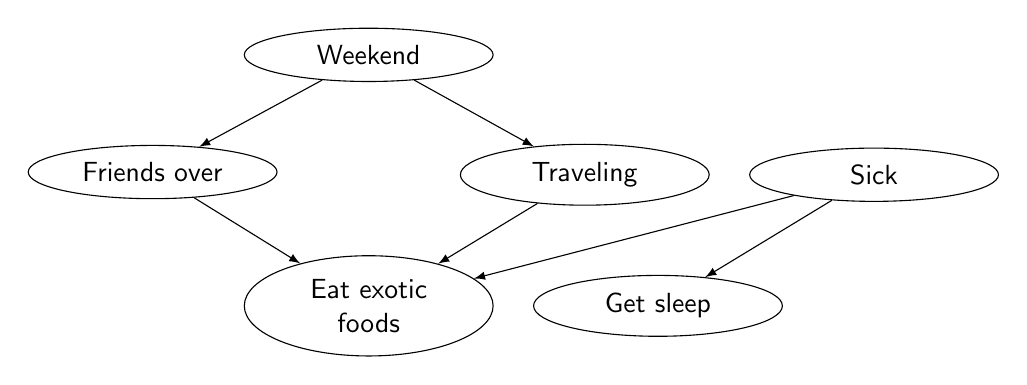
\begin{tikzpicture}[
      node distance=1cm and .5cm,
      bn/.style={draw,ellipse,text width=2cm,align=center}
        ]
      \node[bn] (w) {\attr{Weekend}};
      \node[bn,below right=of w] (t) {\attr{Traveling}};
      \node[bn,right=of t] (s) {\attr{Sick}};
      \node[bn,below left=of w] (f) {\attr{Friends over}};
      \node[bn,below right=of f] (eef) {\attr{Eat exotic foods}};
      \node[bn,right=of eef] (gs) {\attr{Get sleep}};
      \path (w) edge[-latex] (t)
            (w) edge[-latex] (f)
            (f) edge[-latex] (eef)
            (t) edge[-latex] (eef)
            (s) edge[-latex] (gs)
            (s) edge[-latex] (eef);
    \end{tikzpicture}
  \end{center}

\item \textbf{In modified network, $\attr{Friends over}\perp\attr{Get Sleep}$?}  
  YES.  All paths between \attr{Friends over} and \attr{Get Sleep} are blocked:
  \begin{itemize}
    \item Any path via \attr{Weekend} and \attr{Traveling} ends at \attr{Traveling}, which no longer connects to \attr{Get Sleep}.
    \item The only other candidate path is 
    \(\attr{Friends over}\to\attr{Eat exotic foods}\leftarrow\attr{Sick}\to\attr{Get Sleep}\),
    which is blocked by the unconditioned collider \attr{Eat exotic foods}.
  \end{itemize}
  Conditioning on \attr{Eat exotic foods} (the collider) would open that path, making them dependent.
\end{enumerate}
\end{solution}

\newpage
%%%%%%%%%%%%%%%%%%%%%%%%%%%%%%%%%%%%%%%%%%%%%
% Name and Calibration
%%%%%%%%%%%%%%%%%%%%%%%%%%%%%%%%%%%%%%%%%%%%%

\textbf{Name}: Matt Krasnow\\
\textbf{Collaborators and Resources}: Chatgpt for formatting and latex upload

\end{document}
